\chapter{Literature review} \label{chapter2}

\section{YoLo – A brief discussion on v3 and v4 for real-time object detection}
YoLo standing for You Only Look Once is(are) a set of advanced deep learning models for real-time object detection. The focal point for YoLo is that it manages to perform bounding box regression and classification at the same time. The architecture or methodology which separates YoLo and other object detection frameworks is that other sophisticated frameworks (RCNN and even Fast RCNN) attempt to repurpose existing classifiers and localisers to perform object detection. They apply a single model to multiple locations within an image with variations in scale and other properties of the image multiple times. High scoring regions are labelled and classified accordingly. \par

YoLo frameworks take a drastically different approach: they divide the region into a large number of regions (or boxes) and simultaneously apply a single convolutional neural network to the entire image. The bounding boxes and associated probabilities are received at the output. These regions are then weighted according to these probabilities. The reason why this method supersedes other popular methods is that other neural network-based deep learning architectures (such as R-CNN) may end up using multiple network evaluations (in the order of thousands) on a single image that takes up a considerable amount of processing time. Additionally, YoLo models look at the entirety of the image during the detection phase because of which their predictions are based on the global context of the image. Although the differences don’t end here, these fundamental differences are enough to give YoLo a second to third order speed advantage over Fast R-CNN and R-CNN models. \par

The neural network for YoLo along with its entire compilation system is known as Darknet. A typical darknet run on an image, set of images, video or a real-time stream of image content (such as through a webcam) leads to the following three things as output:

\begin{itemize}
  \item The detected classes of objects (e.g. horse, car etc.)
  \item	The prediction confidence (e.g. $0.91$, $0.86$ etc.) and
  \item	The time it took to carry out the prediction or detection (e.g. $6$s, $12$s etc.)
  \item	Sophisticated high-level libraries will also produce the bounding boxes corresponding to each
\end{itemize}

\vspace{-0.1in}

Following is the output when a high-level library like \href{https://pypi.org/project/yolov4/}{yolov4} is used to process an image as shown below.

\begin{figure}[h]

\begin{center}
\begin{subfigure}{0.7\textwidth}
  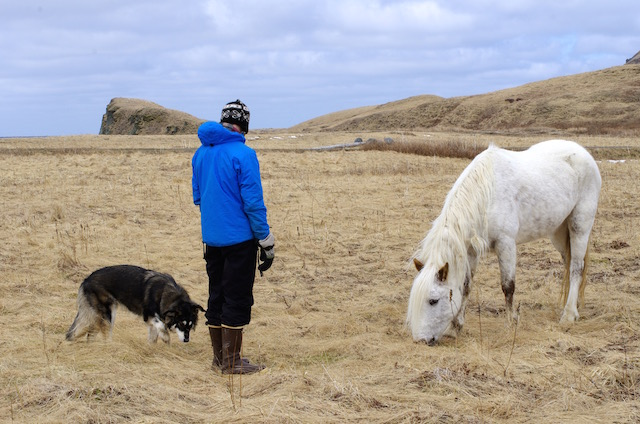
\includegraphics[width=\linewidth, height=5cm]{chapter2/person.jpeg}
  \caption{A sample image taken from the original Darknet \href{https://github.com/AlexeyAB/darknet}{github repository}}
  \label{fig:person_sub1}
 \end{subfigure} \\
 \begin{subfigure}{0.7\textwidth}
  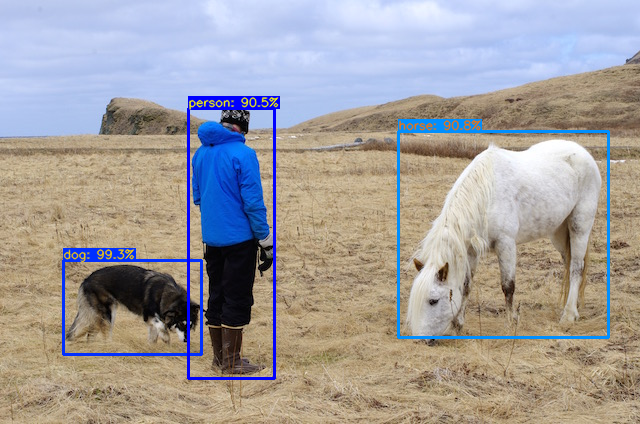
\includegraphics[width=\linewidth, height=5cm]{chapter2/personresult.png}
  \caption{Bounding boxes and detected objects in the image}
  \label{fig:person_sub2}
  \end{subfigure} \\
  \begin{subfigure}{0.7\textwidth}
   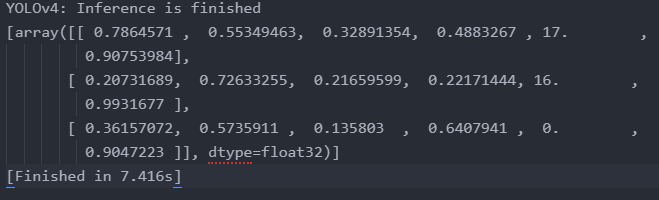
\includegraphics[width=\linewidth, height=5cm]{chapter2/personboxes.png}
   \caption{The bounding box coordinates obtained}
   \label{fig:person_sub3}
 \end{subfigure}

 \caption{A sample Darknet run on an image}
 \label{fig:person_ref}

\end{center}

\end{figure}



\subsection{YoLov3}
Joseph Redmond is credited with designing the original neural network architecture called Darknet. This was made using all low-level languages so that it could be made as flexible as it can be. This architecture went on to produce a series of computer vision wonders in the field of object detection named as YoLo: the original one, v2, v3 and then v4. Even YoLov5 has been developed (the first one to be developed by an organisation as opposed to an individual) at the time of writing this report. However, we won’t be discussing it here since it hasn’t been used in the concerned project. \par

YoLov3 is the first version using an objectivity score for the prediction of bounding boxes. It also proceeds to add further connections to the backbone of the entire architecture. Additionally, detections are also carried out at three levels of granularity which greatly increased the inferencing accuracy on smaller objects as well as objects/ smaller objects placed close to each other. There are some important parts or sections in YoLov3 which proves its robustness to a variety of real-life object detection scenarios. They relate to better bounding box prediction, class prediction, their feature extractor as well better prediction across multiple scales provided in the input. We would be discussing each of them in brief in the following paragraphs. \par

\subsubsection{Bounding box prediction}
Any bounding box in a prediction is represented by a set of four parameters namely $t_x$ and $t_y$: coordinates of the centre of the bounding box and its width and height represented by $t_w$ and $t_h$ respectively. In the event of the top left corner of the bounding box being displaced by $(c_x,c_y)$ respectively, the following overall changes are calculated in the dimensions (assume $p_w$ and $p_h$ are the width and height of the bounding box prior).
\begin{align*}
b_x &=  \sigma(t_x) + c_x \\
b_y &=  \sigma(t_y) + c_y \\
b_w &=  {p_w}e^{t_w} \\
b_h &=  {p_h}e^{t_h}
\end{align*}
Unlike previous systems (or previous YoLo versions), the training phase assigns an objectness score to each bounding box. This score equals one if the current bounding box overlaps a ground truth object to an extent greater than any other previously obtained bounding box. If any previously obtained bounding box doesn’t overlap the ground truth to a greater extent or overlaps only by a certain threshold (say $0.5$ as stated in this paper) then the objectness score is simply zero. Following is a representation of all the important dimensions which are involved in this process.

\begin{figure}
  \centering
  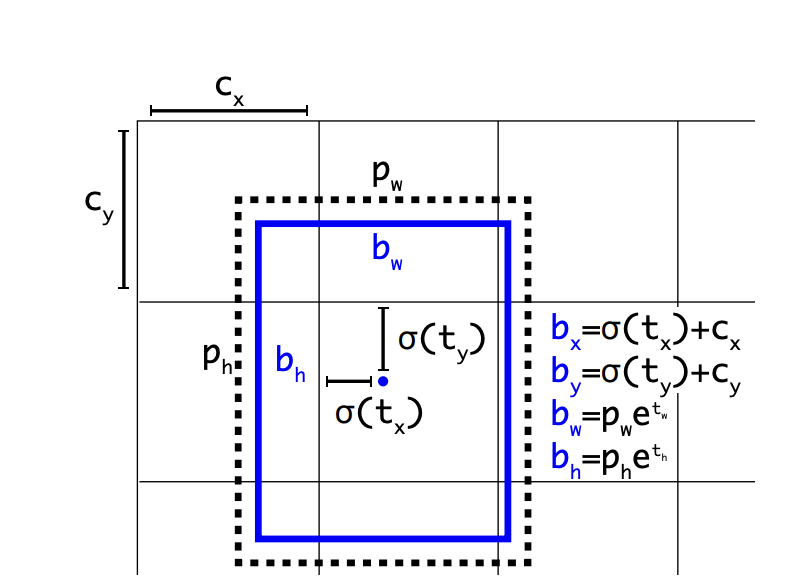
\includegraphics[scale=0.7]{chapter2/bounding_box.png}
  \caption{An illustration showing all the important bounding box dimesnions being used in YoLov3}
  \label{fig:bbox}
\end{figure}

\subsubsection{Class prediction}
SoftMax is one of the most common types of methods used for multi-label classification, however, the method has been leading to decrementing results for the class prediction accuracy in YoLov3 as well as has been unnecessary. Therefore, simple multiple logistic classifiers are being used for the purpose and binary cross-entropy has been used as a loss function. This different approach helped in the case of much larger and more sophisticated datasets such as the Open Images Dataset wherein labels may overlap frequently. SoftMax algorithm assumes that a single bounding box corresponds to exactly one label which is often not the case.

\subsubsection{Feature extraction}
Feature extraction in YoLov3 has been a hybridisation of the one in YoLov2, Darknet – 19 ($19$ convolutional layers) and another residual network. But the most important part of this network is shortcut connections which increase the size of the network significantly, however, continue to supersede ResNet variants in terms of efficiency. Since this leads to a total of $\boldsymbol{53}$ convolutional layers it's named Darknet-53.


\subsection{YoLov4 – improvements over YoLov3}

The fundamental difference between YoLov4 and all its previous variants is that the detector stage has been bifurcated into two distinct sections consisting of a single stage – detector and sparse prediction stage. Following is an illustration of the same.

\begin{figure}[h]
  \centering
  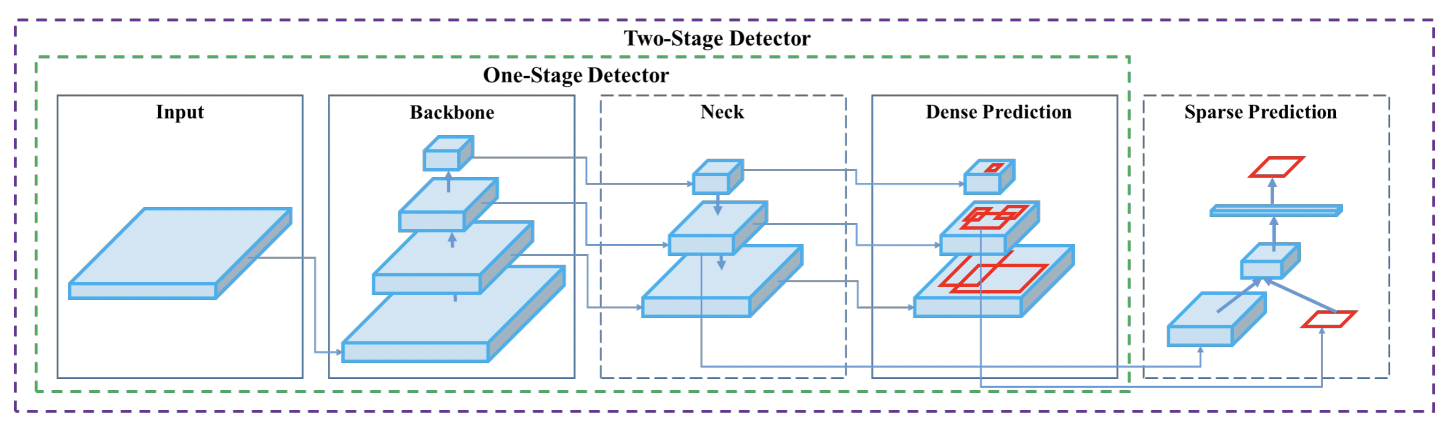
\includegraphics[scale=0.5]{chapter2/detector_stages.png}
  \caption{Two stage detector setup used in YoLov4}
  \label{fig:detector}
\end{figure}

After the initial input phase, we have $\boldsymbol{3}$ main sections as follows.

\subsubsection{Backbone}
This is the common name for the feature extractor section of the entire neural network architecture. It should be noted that all backbones are essentially classification models. With VGG16 being the most common and the earliest deep learning classifiers, SqueezeNet, ShuffleNET and MobileNET are used along with it. These classifiers are meant for the CPU only.

\subsubsection{Neck}
The neck is the common name for a feature aggregator in YoLo frameworks i.e. it collects the feature maps from various sections of the backbone stage. FPN, PAN, NAS-FPN, Fully-connected FPN, BiFPN, ASFF, and SFAM are all examples of feature aggregation blocks used in YoLov4.

\subsubsection{Head}
This is the final stage of the entire framework: a common name for the object detector stage in YoLo frameworks. It should be noted that this stage exclusively tells the region(s) in which (an) object(s) may be located, however, doesn’t tell the class or label to which the object belongs. As stated earlier, these could be a single or two-stage detector, both anchor-based and anchor-free. Some common examples are YOLO, RetinaNet, SSD, Faster – RCNN etc.

As the number of examples in each stage shows, a typical YoLov4 framework can be implemented in any combination of input, backbone, neck and head. When there are such a large number of combinations possible, the best architecture should be an optimal combination of all the sections. This optimal choice would alone make it superior to YoLov3 in terms of \textbf{performance and accuracy}. This optimal combination should be arrived at by looking at the following parameters:

\begin{itemize}
\item Input resolution of images and their size
\item Number of convolutional layers
\item Number of parameters (hyperparameters) to be optimised
\item Number of output layers or filters
\item YoLov4 also provides something known as \textit{Bag of Specials} and \textit{Bag of Freebies} which are methods or functions for increasing the respective fields and mappings between backbone levels to detector levels. This gives us another region wherein optimisation can be done.

\end{itemize}

\newpage

The final architecture that was deemed optimal for YoLov4 is as follows (with backbone, neck and head in order).

\begin{figure}[h]
  \centering
  \begin{tikzpicture}[node distance=4cm]
    \node (backbone) [process] {CSPDarknet53};
    \node (neck) [process, right of=backbone] {SSP $+$ PANet};
    \node (head) [process, right of=neck] {YoLov3};
    \draw [arrow] (backbone) -- (neck);
    \draw [arrow] (neck) -- (head);
  \end{tikzpicture}
  \caption{The final architecture presented in the paper}
  \label{fig:final_arch}
\end{figure}

A couple of other combinations were derived but the FPS of the above combination superseded everything else.  A summary of the FPS values of a couple of other possibilities is given below. Now we are going to see some special sections of the architecture (but are not limited to) in detail which make it more efficient than YoLov3.

\begin{table}[h]
 \def\arraystretch{1.5}
 \centering
 \caption{Neural network parameters for image recognition for $512 \times 512$ network resolution}
 \begin{tabular}{|c|c|c|c|c|c|}
  \hline
  Backbone model & Receptive field size & Parameters & Average layer size & BFLOPs & FPS\\
  \hline
  CSPResNext50 & $425 \times 425$  & $20.6$ mn & $1058$ K & $31$ & $62$                   \\
  \hline
  CSPDarknet53 & $725 \times 725$ & $27.6$ mn & $950$ K & $52$ & $66$                        \\
  \hline
  EfficientNet & $1311 \times 1311$ & $12$ & $668$ K & $11$ & $26$                        \\
  \hline
 \end{tabular}
 \label{tab:mccons}
\end{table}


\subsubsection{Cross Stage Partial connection (CSP)}
In any large neural network-based architecture, it is common for the last and the second to last layers to lose out on a lot of contextual features seen by the initial layers. A way out of this is to introduce the concept of skip connections so that the backpropagation of gradients to the initial layers can be done easily. DenseNet was initially considered for this but it had skip connections between every other layer which proved to be inefficient. So, the researchers stuck with their initial choice of CSPResNext50 and the CSPDarknet53 as far as the architecture is concerned. Following is an illustration of the same.

\begin{figure}[h]
  \centering
    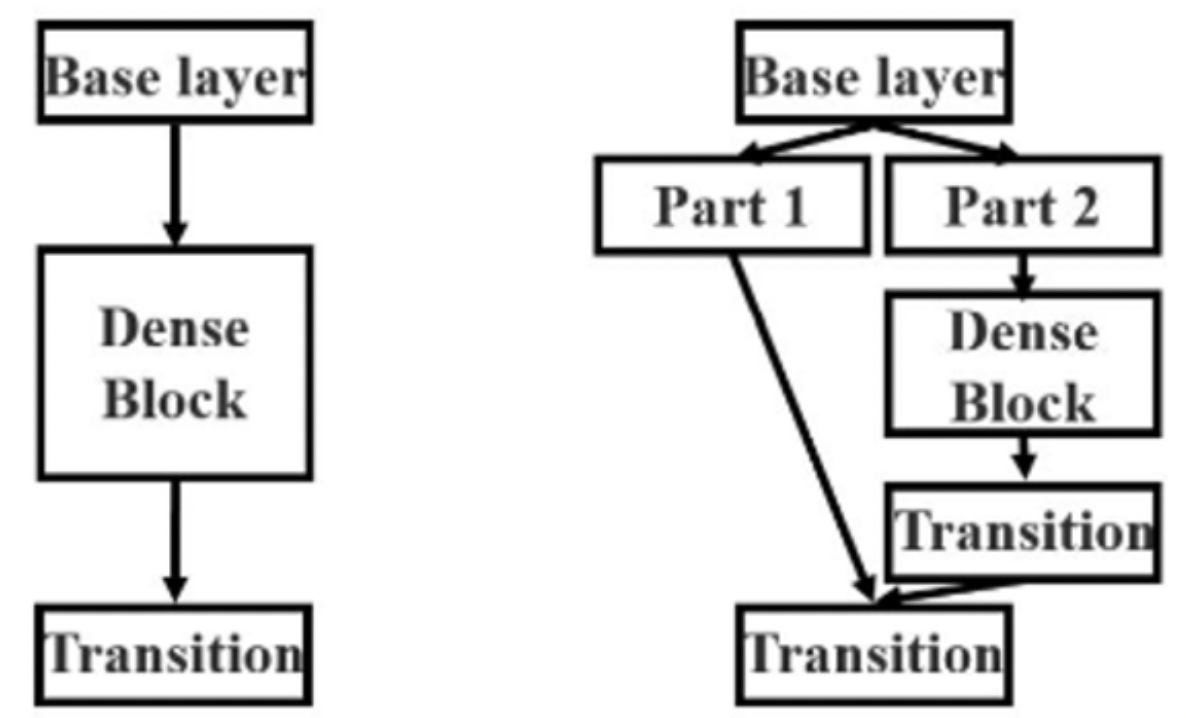
\includegraphics[scale=0.5]{chapter2/dense_architectures.png}
  \caption{The two possible dense architectures: DenseNet and CSPDensnet}
  \label{fig:dense_arch}
\end{figure}

\subsubsection{Self-Adversarial Training (SAT)}
Deep learning is very much susceptible to adversarial data so YoLov4 uses SAT to introduce precise amounts of perturbation in the data such that the predicted label stays the same as the original label. This helps it easily achieve good accuracies for even augmentations of simple images.

All these discussions prove the benefits and advantages of YoLov4 over YoLov3 and hence it's choice for the project. As always, all things are better quantified in a graph of MAP versus execution time as shown below.

\begin{figure}[h]
  \centering
  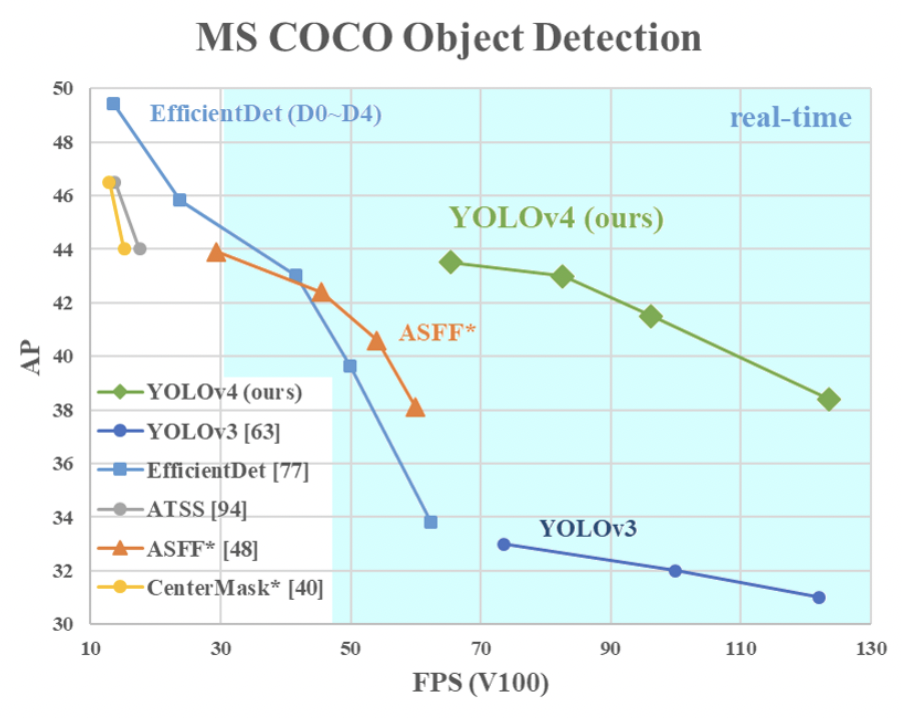
\includegraphics[scale=0.8]{chapter2/v3v4.png}
  \caption{YoLov4 vs other state of the art object detectors}
  \label{fig:v3_vs_v4}
\end{figure}


\section{Performance metrics for evaluating object detection models \cite{Koech2020}}

The entirety of this report deals with a large number of performance metrics used to evaluate a variety of ML/DL models. Some are popular and have been used to evaluate such models for a long time while some metrics are empirical in nature because their output is a combination of a variety of models dealing with different classes of inputs and outputs which are working together. However, we would be specifically discussing metrics used for the evaluation of the performance of object detection models in this section.
\subsection{Intersection over Union (IoU)}
This metric equals the amount of overlap between the ground truth denoted by $g_t$ and the predicted value by a particular model i.e. prediction denoted by $p_d$. It is to be noted that since this value is a ratio, it is a fraction consisting of numerator and denominator areas in appropriate units. Mathematically, it is given by
\begin{equation}
\centering
IoU = \frac{area({g_{t}}\cap{ p_{d }})}{area({g_{t}}\cup{ p_{d }})}
\end{equation}
As it is very obvious for any arbitrary situation $0 \leqslant $ IoU $\leqslant 1$ wherein $0$ corresponds to a null overlap and $1$ corresponds to a full overlap. However, in almost all ML/DL models we don’t go for such strict definitions rather we define what we call the IoU at $\alpha$ (or abbreviated as IoU@$\alpha$). This means any value of IoU $\geqslant \alpha$ is considered a true positive whereas any value otherwise is considered a true negative. \par

Before we go ahead and define the next important metric we need to know a couple of different terms as stated below:
\begin{itemize}
 \item \textbf{Precision} – The degree to which a model can identify only the relevant objects. It is simply the ratio of true positives and all the detections made by the model. It is given by
\begin{equation}
\centering
P = \frac{True \ positives}{All \ detections \ made \ by \ the \ model}
\end{equation}
 \item \textbf{Recall} – The degree to which the model can detect all true positives amongst all ground truths. Mathematically, it is the ratio of the number of true positives and all ground truths and is given by
\begin{equation}
\centering
R = \frac{True \ positives}{All \ ground \ truths}

\end{equation}

\textbf{A good model has a high precision as well as high recall}.

 \item \textbf{Precision–recall curve} – It is simply the plot of the variation of precision and recall against the variation of confidence values. A good model will give high precision values even when confidence is varied significantly.
 \item \textbf{Average precision} – When the area under the precision-recall curve is calculated at the IoU@$\alpha$ threshold then we get this value. Formally, it is defined using the following integral.
\begin{equation}
\centering
AP@\alpha = \int\limits_{0}^{1} p(r) \ \mathrm{d} r
\end{equation}

\end{itemize}

Now we are at a stage where we can understand the next important metric

\subsection{Mean Average Precision (mAP)}
For each class, the average precision as defined above is calculated. This roughly translates to No. of average precision values $\approx$ No. of classes. When the average of these average precision is taken we get what we know as the mean average precision. For $n$ classes we can simply calculate it as follows:
\begin{equation}
\centering
mAP@\alpha = \frac{1}{n} \sum_{i=1}^{n} AP_{i}
\end{equation}


\section{Guidelines for a good YoLo project}
The following rules for a good project using YoLo are mere \textit{thumb – rules} and are not some strict guidelines to be followed and should be evaluated on a case to case basis for every project. Additionally, it should be noted that such rules may not be applicable for implementation in every object detection project. The following rules are bifurcated into those undertaken during the training and those in the testing (detection) phase.

\subsection{For training}

\begin{enumerate}
  \item The values of {\fontfamily{qcr}\selectfont random} should be set to $1$ in your  {\fontfamily{qcr}\selectfont .cfg} file which allows training for multiple image or video resolutions simultaneously.
  \item Every distinct object that is liable for detection must have an appropriate label in the dataset.
  \item Precision may be increased by keeping the height and width of images or video frames as a multiple of $32$.
  \item The training dataset should be such that every object to be detected corresponds to an exactly similar object in the training dataset. Similarity should be in terms of size, no. of classes to be detected ($c$), overall spatial orientation, overall illumination, augmentation (if any) etc. \par

  If the size of the training dataset is $N$ and the no. of classes is stated as above then training must run for at least $Nc$ iterations.
  \item Training datasets should have as many \textbf{positive} examples as there are \textbf{negative} examples (i.e. images which don’t have any object to be detected). Such negative examples shall return no bounding boxes when the detection or testing run is executed. These ensure an equal sensitivity of the model to both types of images as well as eliminate a lot of post-processing operations.
  \item Sometimes it is desirable to run your detections with the {\fontfamily{qcr}\selectfont -show\_imgs} option at the end so that it can be manually verified whether the predicted bounding boxes are correct or not. Seeing the detections and detecting some anomaly could be a direct implication of training runs going wrong or some inherent problem in the dataset.
\end{enumerate}


\subsection{For testing or detection}

\begin{enumerate}
  \item Increase network resolution in the same way as mentioned in 1. c.
  \item It should be noted that retraining is not required in the event of loss in your dataset or any other unintended corruption. Only the \textit{darknet} command should be available which can be used to perform detections using the pre-trained {\fontfamily{qcr}\selectfont .weights} file which was trained on the $416 \times 416$ resolution images.
  \item To further enhance the accuracy, dataset training must proceed onto higher multiples of  $32$ such as $608 \times 608$ or $832 \times 832$. In the event of a memory overflow ({\fontfamily{qcr}\selectfont Out of memory}), {\fontfamily{qcr}\selectfont subdivisions} in your {\fontfamily{qcr}\selectfont .cfg} file must be increased from $16$ to $32$ to $64$ and so on.
\end{enumerate}
